\documentclass[12pt]{article}

% Paquetes
\usepackage[utf8]{inputenc}
\usepackage[spanish]{babel}
\usepackage{milibreria}

% Título
\title{}
\author{Tú Nombre}
\date{\today}

\begin{document}

\textcolor{black}{\rule{0.9\linewidth}{1.5mm}} \par
\vspace*{3cm}
                \begin{minipage}{0.9\textwidth}
                    \centering
                    {\Large {\textbf{Desarrollo de un Sistema de Monitoreo en Tiempo Real para Optimizar el Rendimiento Académico en el colegio Aplicación: Enfoque en Asistencia, Atención y Emociones Estudiantiles}}}\par
                \end{minipage}
\vspace*{3cm}
\par \textcolor{black}{\rule{0.9\linewidth}{0.5mm}} \par

\href{mailto:dlarotap@est.unap.edu.pe}{\textbf{David Larota *}}  \\
\href{https://maps.app.goo.gl/y7MUTXXG2xKvnvZVA}{Universidad Nacional del Altiplano}\\
\href{mailto:dlarotap@est.unap.edu.pe}{dlarotap@est.unap.edu.pe}\\


\begin{abstract}

\end{abstract}

\newpage
\tableofcontents

\newpage
\section{Planteamiento de teórico de la Investigación}
\subsection{Exposición de la Situación Problemática}
Al observar la dinámica en el aula del Colegio Aplicación, pude identificar una situación problemática relacionada con la falta de atención de algunos estudiantes durante las clases. En diversas ocasiones, noté que varios alumnos parecían desconectados o distraídos, lo que podría afectar negativamente su rendimiento académico. El profesor, a su vez, se encontraba ocupado dictando la materia y no siempre tenía la capacidad de percatarse de la falta de atención de manera inmediata.
\espacio
Esta carencia de atención puede atribuirse a diversos factores, como problemas personales, falta de interés en el contenido, o incluso la presencia de distracciones en el entorno escolar.
\cite{atencion3}
\subsection{Formulación del problema}
La situación problemática se centra en las limitaciones de los métodos tradicionales para monitorear el rendimiento de los estudiantes en el aula, especialmente en lo que respecta a métricas críticas como la asistencia, los niveles de atención y el estado emocional. Estas limitaciones dificultan la capacidad de los instructores para gestionar eficazmente la dinámica del aula, lo que puede llevar a resultados académicos subóptimos. Por lo tanto, el estudio busca desarrollar un sistema innovador de visión en tiempo real que utilice modelos YOLOv7 para monitorear las emociones, la asistencia y los niveles de atención de los estudiantes, con el objetivo de proporcionar información en tiempo real sobre métricas críticas que los métodos tradicionales no pueden capturar
\begin{figure}[!h]
    \centering
    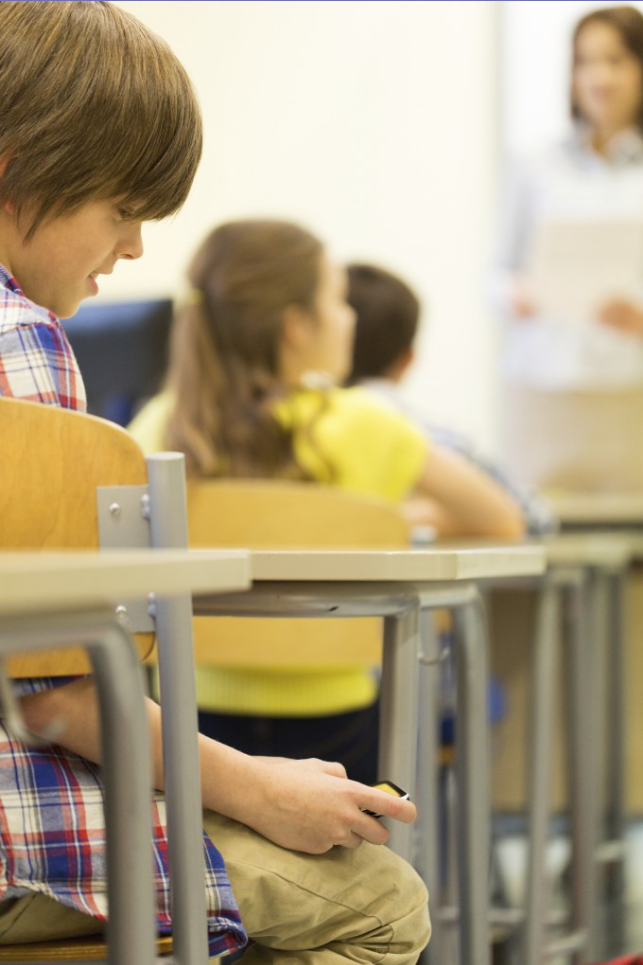
\includegraphics[width=0.3\textwidth]{images/falta_atencion.png}
    \caption{alumno por falta de atención} 
\end{figure}
\subsubsection{interrogante general} 
¿Cómo se puede desarrollar un sistema innovador de visión en tiempo real que utilice modelos YOLOv7 para monitorear las emociones, la asistencia y los niveles de atención de los estudiantes en el aula, con el fin de proporcionar información en tiempo real sobre métricas críticas que los métodos tradicionales no pueden capturar?
\subsubsection{interrogante especifica}
¿y cómo este sistema podría mejorar el rendimiento tanto de los instructores como de los estudiantes a nivel académico?
\subsection{Justificación del problema}
La problemática de los adolescentes notificados por problemas de conducta y aprendizaje, según la Defensoría de la Mujer, del Niño y del Adolescente, destaca la necesidad urgente de comprender y abordar estos desafíos. En este sentido, la falta de estrategias efectivas para mejorar la situación de los estudiantes se convierte en un problema relevante que merece una investigación detallada.
 \espacio
Además, al analizar las estrategias de aprendizaje en estudiantes con atención semipresencial, como se evidencia en el caso del CEBA José Antonio Encinas - Puno, se identifica la importancia de mejorar y adaptar las metodologías educativas para optimizar el rendimiento académico.
\cite{justificacion}
\subsection{Objetivos de la Investigación}
\subsubsection{Objetivo General}
Optimizar el rendimiento académico en el colegio mediante la implementación de un sistema de monitoreo en tiempo real que se enfoque específicamente en mejorar los índices de asistencia, niveles de atención y gestión emocional de los estudiantes.
\subsubsection{Objetivos específicos}
\begin{itemize}
    \item Diseñar Indicadores de Asistencia
    \item Implementar un Sistema de Monitoreo en Tiempo Real
    \item Evaluar Niveles de Atención
    \item Integrar Reconocimiento Emocional
    \item Generar Informes y Estadísticas
    \item Capacitar al Personal Educativo
\end{itemize}

\subsection{Factibilidad y viabilidad de la investigación }
\subsubsection*{Factibilidad Técnica}
\textbf{Infraestructura Tecnológica:} Evaluar la disponibilidad y capacidad de la infraestructura tecnológica en el colegio para implementar el sistema de monitoreo.\\
\textbf{Conocimientos Técnicos:} Analizar el nivel de conocimientos técnicos del personal y estudiantes para garantizar una adopción efectiva del sistema.\\
\textbf{Compatibilidad:} Verificar la compatibilidad del sistema con las plataformas y dispositivos existentes.
\subsubsection*{Factibilidad Operativa}
\textbf{Proceso de Implementación:} Determinar la viabilidad del proceso de implementación, considerando posibles interrupciones en las actividades académicas.\\
\textbf{Capacitación del Personal:} Evaluar la necesidad y factibilidad de capacitación para el personal encargado de utilizar y gestionar el sistema.
\subsubsection{Factibilidad Económica}
\textbf{Presupuesto:} Estimar los costos asociados con el desarrollo e implementación del sistema, incluyendo software, hardware, capacitación y mantenimiento.\\
\textbf{Retorno de Inversión:} Analizar el retorno de inversión esperado a través de mejoras en el rendimiento académico y eficiencia operativa.
\subsubsection*{Factibilidad Legal y Ética}
\textbf{Cumplimiento Normativo:} Verificar que el sistema cumpla con las normativas y regulaciones educativas y de protección de datos.\\
\textbf{Consideraciones Éticas:} Evaluar las implicaciones éticas del monitoreo, garantizando la privacidad y consentimiento de los estudiantes.
\subsubsection*{Viabilidad del Estudio}
\textbf{Relevancia:} Confirmar la relevancia y necesidad del sistema de monitoreo en el contexto educativo del colegio.\\
\textbf{Apoyo Institucional:} Obtener el respaldo y compromiso de la institución educativa para garantizar el éxito del estudio.    

\subsection{Hipótesis, Variables e indicadores}
\subsubsection{Hipótesis general}
Se presume que la implementación exitosa de un "Sistema de Monitoreo en Tiempo Real para Optimizar el Rendimiento Académico en el colegio Aplicación: Enfoque en Asistencia, Atención y Emociones Estudiantiles" conducirá a mejoras significativas en la asistencia, atención y rendimiento académico de los estudiantes.
\subsubsection{Hipótesis especifica}
Se supone que la implementación del sistema de monitoreo mejorará la asistencia estudiantil al proporcionar alertas tempranas y recordatorios automáticos a los padres y estudiantes sobre la importancia de la asistencia regular.\\
Se presume que el enfoque en la atención, a través del monitoreo continuo de la participación y la interacción en el aula, contribuirá a un aumento en la retención de información y, por lo tanto, mejorará el rendimiento académico.\\
Se hipotetiza que la evaluación en tiempo real de las emociones estudiantiles permitirá a los educadores identificar factores emocionales que afectan el rendimiento, facilitando intervenciones específicas para mejorar el bienestar emocional y el aprendizaje.\\
Se supone que la aplicación del sistema de monitoreo en tiempo real facilitará la comunicación entre padres, estudiantes y educadores, fomentando un entorno colaborativo que respalda el éxito académico.
\subsubsection{Variable(s)}
\textbf{Sistema de Monitoreo en Tiempo Real:} La implementación de un sistema de monitoreo en tiempo real permite obtener información instantánea y precisa sobre el comportamiento de los estudiantes, lo que facilita una intervención rápida y eficiente.\\
\textbf{Optimizar el Rendimiento Académico:} Mejorar el rendimiento académico es el objetivo principal de cualquier institución educativa. La recopilación de datos en tiempo real y su análisis permiten identificar áreas de mejora y personalizar estrategias educativas para cada estudiante.\\
\textbf{Enfoque en Asistencia:} La asistencia regular a las clases es esencial para el éxito académico. Monitorear la asistencia en tiempo real ayuda a identificar patrones y problemas relacionados con la puntualidad, lo que puede abordarse proactivamente.\\
\textbf{Enfoque en Atención:} La atención activa en el aula es crucial para el aprendizaje efectivo. Monitorear la atención permite a los educadores adaptar sus métodos de enseñanza y brindar apoyo adicional a los estudiantes que lo necesiten.\\
\textbf{Enfoque en Emociones Estudiantiles:} Las emociones juegan un papel significativo en el proceso de aprendizaje. Comprender y abordar las emociones estudiantiles contribuye al bienestar emocional, creando un entorno propicio para el aprendizaje y mejorando la salud mental de los estudiantes.
%\subsubsection{Dimensiones }
\subsubsection{Indicadores}
\subsubsection*{Sistema de Monitoreo en Tiempo Real}
Frecuencia de actualización de datos.\\
Tiempo de respuesta del sistema.\\
Nivel de accesibilidad y usabilidad del sistema.
\subsubsection*{Optimización del Rendimiento Académico}
Mejora en las calificaciones promedio.\\
Reducción de la tasa de reprobación.\\
Aumento en la participación y colaboración estudiantil.
\subsubsection*{Asistencia}
Tasa de asistencia diaria y semanal.\\
Niveles de puntualidad de los estudiantes.\\
Frecuencia de alertas tempranas de ausencias.
\subsubsection*{Atención}
Medición de la participación activa en clases.\\
Evaluación de la retención de información.\\
Identificación de patrones de distracción.
\subsubsection*{Emociones Estudiantiles}
Registro de expresiones emocionales durante las clases.\\
Evaluación de encuestas sobre el estado emocional de los estudiantes.\\
Análisis de patrones emocionales y su relación con el rendimiento académico.

%\subsubsection{Operacionalización de la(s) variable(s)}
%\lipsum[1]
%\subsubsection{Definición conceptual de la(s) variable(s)}
%\lipsum[1]

\section{Marco Teórico }
\subsection*{Teoría de la Educación}

La teoría de la educación sostiene que la participación activa de los estudiantes es esencial para un aprendizaje efectivo. El monitoreo en tiempo real de la asistencia y atención puede promover la participación, mejorando así el rendimiento académico.
\subsection*{Tecnología Educativa}

Investigaciones sobre tecnologías educativas resaltan la eficacia de los sistemas de monitoreo para mejorar la interacción en el aula. La implementación de herramientas tecnológicas puede optimizar la gestión académica y facilitar la retroalimentación instantánea.
\subsection*{Teoría del Aprendizaje}

Desde la perspectiva de la teoría del aprendizaje, la atención y el estado emocional impactan la retención de información. Monitorear las emociones estudiantiles y la atención puede ayudar a adaptar el proceso de enseñanza para optimizar el aprendizaje.
\subsection*{Psicología Educativa}

La psicología educativa subraya la importancia de abordar las emociones para mejorar el rendimiento académico. Un sistema que monitorea las emociones estudiantiles puede proporcionar insights valiosos para el diseño de estrategias pedagógicas efectivas.
\subsection*{Sistemas de Monitoreo y Gestión Escolar}

La literatura sobre sistemas de monitoreo en entornos escolares destaca su contribución a la eficiencia administrativa. Integrar aspectos de asistencia, atención y emociones en un solo sistema puede mejorar la gestión escolar de manera integral.
\subsection*{Inteligencia Artificial y Análisis de Datos}

La aplicación de inteligencia artificial y análisis de datos en la educación permite una evaluación más precisa de patrones de asistencia, atención y emociones. Esto facilita la toma de decisiones informadas para la mejora continua del rendimiento académico.
\subsection{Antecedentes de la investigación } %(Internacional, Nacional y local)
\subsubsection*{Antecedentes Locales}
Sistema de Monitoreo de Rendimiento Académico en la I.E. Pedro A. Lavarte:
Villalobos Yarihuamán (2018) desarrolló un Sistema Web para el monitoreo de rendimiento académico en los cursos de estudiantes de primer grado de secundaria en la I.E. Pedro A. Lavarte. Este antecedente local proporciona un contexto específico sobre el monitoreo académico a nivel escolar.
\subsubsection*{Antecedentes Nacionales}
Reconocimiento a Estudiantes por Desarrollo de Sistema Logístico de Monitoreo Remoto:
En la Universidad Católica de Santa María, durante el inicio del Año Académico 2021, estudiantes desarrollaron el "Sistema Logístico de Monitoreo Remoto en Tiempo Real, de la Cadena de Frío para las Vacunas Contra el Coronavirus." Este proyecto destaca la importancia de la monitorización en tiempo real, aunque se centra en la logística y no específicamente en el rendimiento académico.
 
\subsubsection*{Antecedentes Internacionales}
El artículo tiene como objetivo mejorar la comunicación e interacción dentro de las instituciones educativas a través de una aplicación móvil. Se destaca la importancia de la base de datos como fuente esencial para la integración y recopilación de información en el sector educativo. Se considera cada institución como una entidad, donde todos los individuos que interactúan con ella conforman la población. La premisa fundamental es que esta población necesita estar conectada y comunicada para prosperar.

\subsection{teóricas científicas }%(Marco teórico esquemático)
\subsubsection*{Estrategias Educativas Innovadoras} Se propone el uso de estrategias educativas innovadoras como herramienta para elevar el rendimiento académico %[1].

\subsubsection*{Relación entre Metacognición y Rendimiento Académico} Se analiza la relación entre la metacognición y el rendimiento académico, especialmente en áreas específicas como la química general en estudiantes universitarios %[2].

\subsubsection*{Optimización del Rendimiento Académico en Estudiantes de Estomatología} Se aborda la optimización del rendimiento académico en estudiantes de Estomatología, destacando la importancia de estrategias específicas %[3].

\subsubsection*{Teorías Subjetivas en Docentes} Analiza las teorías subjetivas en docentes y su impacto en la eficacia de una institución escolar, poniendo de relieve la influencia del pensamiento del profesor %[4].

\subsubsection*{Teoría Científica del Rendimiento Académico en Enseñanza Primaria} Explora teorías científicas, validez externa y teorías de alcance intermedio relacionadas con el rendimiento académico en la enseñanza primaria %[5].
\subsection{Marco conceptual }%(definición de términos)
\subsubsection*{Rendimiento Académico}

Se refiere al nivel de logro y éxito que un estudiante alcanza en sus actividades educativas y evaluaciones.
Incluye aspectos como calificaciones, resultados en exámenes y participación en actividades académicas.
\subsubsection*{Inteligencia Emocional}

Comprende la capacidad de reconocer, comprender y gestionar las propias emociones y las de los demás.
Incluye componentes como la autoconciencia, autorregulación, motivación, empatía y habilidades sociales.
\subsubsection*{Relación entre Rendimiento Académico e Inteligencia Emocional}

Existe la hipótesis de que las habilidades de inteligencia emocional pueden influir positivamente en el rendimiento académico.
La capacidad para manejar el estrés, establecer relaciones efectivas y mantener la motivación podría contribuir al éxito académico.
\subsubsection*{Factores Mediadores}

Se consideran factores que podrían mediar la relación, como el bienestar psicológico, la adaptabilidad emocional y la resiliencia.
Estos factores podrían influir tanto en el aspecto emocional como en el rendimiento académico.
\subsubsection*{Estudio de Investigación}

El marco conceptual se aplica a un proyecto de investigación específico que busca establecer la relación entre el rendimiento académico y la inteligencia emocional de los estudiantes.
%\subsection{Descripción de la unidad investigada  }%(opcional)


\section{Procesamiento Metodologico de la Investigación}
\subsection{Metodología del estudio}
\subsubsection{  Diseño de la investigación}
\lipsum[1]
\subsubsection{  Tipo de investigación}
\lipsum[1]
\subsubsection{  Enfoque de investigación}
\lipsum[1]
\subsubsection{  Alcance de la Investigación (nivel)}
\lipsum[1]
\subsubsection{  Linea de investigación}
\lipsum[1]
\subsection{Unidad de estudio}
\subsubsection{Ubicación espacial o ámbito de investigación}
Ubicación de la investigación, la investigación se realizo en la ciudad de Puno, Perú queda al sur del Perú cerca a Bolivia 

\subsubsection{Población}
\lipsum[1]
\subsubsection{Muestra}
\lipsum[1]
\subsubsection{Temporalidad o tiempo social}
\lipsum[1]
\subsection{Técnicas e instrumentos de investigación}
\lipsum[1]
\subsubsection{Técnicas}
\lipsum[1]
\subsubsection{Instrumentos}
\lipsum[1]
\subsubsection{Validación y confiabilidad de los instrumentos}
\lipsum[1]
\subsection{Estrategias de recolección de datos}
\lipsum[1]
\subsubsection{Procedimientos }
\lipsum[1]
\subsubsection{Procesamiento de la información}
\lipsum[1]
\section{ASPECTOS ADMINISTRATIVOS}
\lipsum[1]
\subsection{Recursos humanos}
\lipsum[1]
\subsection{Recursos materiales}
\lipsum[1]
\subsection{Recursos económicos}
\lipsum[1]
\subsection{Recursos financieros}
\lipsum[1]
\section*{CRONOGRAMA DE TRABAJO}
\lipsum[1]

\cite{prueba}

\newpage
\section{Referencias}
\bibliographystyle{apacite}
\bibliography{referencias.bib}


\end{document}
